
The $\delta m_W^{\scriptsize\textrm{PDF}}$ shift for each PDF set is evaluated for the
Tevatron experiments and ATLAS using the precise NNLO {\textsc{Wj-MiNNLO}} calculation.  
The resulting shifts are are compared to those from the NLO
{\textsc{W\_ew-BMNNP}} and {\textsc{Resbos}} calculations, and the differences are typically
within the statistical precision of the comparison.  For LHCb the PDF shift is determined
with a direct fit to the data as in the original measurement.

All experimental measurements include an {\it in situ} constraint on \pTZ~and/or \pTW.  We
preserve these constraints by reweighting the relevant boson \pT distribution for each PDF
set to match that used in the measurement.  For the Tevatron experiments \pTW~is reweighted,
while in the case of ATLAS \pTZ~is reweighted since the lower recoil resolution does not
provide a significant \pTW~constraint from the data.  For LHCb a constraint on \pTW~is applied
as part of the direct fit to the data for each PDF set.

For each PDF set $\delta m_W^{\scriptsize\textrm{PDF}}$ is evaluated using a common boson $\pT$~distribution
across PDFs separately for each experiment.  For the Tevatron experiments the $W$ boson $\pT$~is
reweighted to match that of the original measurement, due to the observed agreement between the measured
recoil distribution and the model.  In the case of ATLAS the $Z$-boson $\pT$~is reweighted to match the
original measurement, since the lower recoil resolution does not provide a significant $W$-boson
$\pT$ constraint from the data.
For LHCb the PDF shift is determined with a direct fit to the
data as in the original measurement, including constraints on $\pTW$ and the most relevant polarization
coefficient.

In order to facilitate the evaluation of uncertainty correlations, Hessian eigenvector sets are 
used.  The upper and lower uncertainties are taken to be 
\begin{eqnarray}
\sigma_{m_{W}^+} = \left[\sum_i \left({\sigma_{m_{W}^i}}\right)^2\right]^{1/2} \textrm{ if } \sigma_{m_{W}^i}>0 
~\,\,\,\textrm{and} \,\,\,\,\,\, \nonumber \\
\sigma_{m_{W}^-} = \left[\sum_i \left({\sigma_{m_{W}^i}}\right)^2\right]^{1/2} \textrm{ if } \sigma_{m_{W}^i}<0,
\end{eqnarray}
where $i$ runs over the uncertainty sets.  The uncertainties are symmetrized according to 
$\sigma_{m_{W}} = (\sigma_{m_{W}^+} + \sigma_{m_{W}^-})/2$.  For CTEQ PDF sets the translation from 90\% C.L. 
to 68\% C.L. assumes a gaussian distribution, i.e. a division by 1.645.  The effect of each PDF eigenset 
is correlated across experiment or measurement category, and its contribution to the covariance between 
any two measurements $\alpha$ and $\beta$ is given by
$C^i_{\alpha\beta} = \sigma_{m_{W\alpha}^i} \sigma_{m_{W\beta}^i}$.
Accounting for all eigensets of a given PDF, the total uncertainty covariance and the corresponding 
uncertainty correlation are calculated as
\begin{equation}
C^{\scriptsize\textrm{PDF}}_{\alpha\beta} = \sum_i C^i_{\alpha\beta},~\,\,\,\textrm{and}\,\,\,\,\rho_{\alpha\beta} = 
\frac{\sum_i \sigma_{m_{W\alpha}^i} \sigma_{m_{W\beta}^i}}{\sigma_{m_{W\alpha}}\sigma_{m_{W\beta}}}.
\end{equation}

Tables~\ref{tab:shiftmT} and \ref{tab:shiftpTlmet} show $\delta m_W^{\scriptsize\textrm{PDF}}$ for each PDF set and each 
experiment using distributions based on the transverse mass and the lepton or neutrino $p_T$, respectively.  
For simplicity the ATLAS shifts are shown inclusively in lepton $\eta$, though separated by boson charge.
The PDF uncertainties for each measurement are shown in Table~\ref{tab:pdfunc}, and the correlation 
matrices for the the most recent PDF sets are shown in Fig.~\ref{fig:pdfcorr}.  Correlation matrices for
older sets are provided in the Appendix.

\begin{table}[!tbp]
  \centering 
\begin{tabular}{lrrrr}
\hline \hline 
              PDF set  &        D0   &            CDF &  ATLAS $W^+$ &  ATLAS $W^-$ \\
\hline
              CTEQ6    &     $-14.6$ &            0.0 &           -- &           -- \\ 
              CTEQ6.6  &         0.0 &           14.2 &           -- &           -- \\ 
              CT10     &      $-0.5$ &           14.3 &          0.0 &          0.0 \\ 
              CT14     &      $-8.7$ &            5.2 &       $-0.5$ &       $-7.6$ \\ 
              CT18     &      $-7.5$ &            6.5 &         13.4 &       $-5.5$ \\ 
              ABMP16   &     $-17.9$ &         $-2.4$ &      $-25.7$ &       $-7.9$ \\ 
              MMHT2014 &     $-10.1$ &            4.5 &       $-3.6$ &          9.1 \\ 
              MSHT20   &     $-12.9$ &            2.5 &      $-22.3$ &          4.2 \\ 
              NNPDF3.1 &      $-1.0$ &           13.1 &      $-14.6$ &       $-6.3$ \\ 
              NNPDF4.0 &         6.2 &           20.1 &      $-23.3$ &          4.3 \\ 
\hline \hline
\end{tabular}
  \caption{Values of $\delta m_W^{\scriptsize\textrm{PDF}}$ in MeV for each PDF set using the \mT~fit
  distribution, determined using the {\textsc{Wj-MiNNLO}} calculation.
}
\label{tab:shiftmT}
\end{table}

\begin{table*}[!tbp]
  \centering 
\begin{tabular*}{\linewidth}{l @{\extracolsep{\fill}}rrrrrrr}
\hline \hline 
              PDF set  & D0 \pTl & D0 \met & CDF \pTl &    CDF \met     & ATLAS $W^+$ &  ATLAS $W^-$ & LHCb    \\
\hline
              CTEQ6    & $-17.0$ & $-17.7$ &      0.0 &             0.0 &          -- &          -- & -- \\ 
              CTEQ6.6  &     0.0 &     0.0 &     15.0 &            17.0 &          -- &          -- & -- \\ 
              CT10     &     0.4 &  $-1.3$ &     16.0 &            16.3 &         0.0 &         0.0 & -- \\ 
              CT14     &  $-9.7$ & $-10.6$ &      5.8 &             6.8 &        -1.2 &      $-5.8$ & 1.1 \\ 
              CT18     &  $-8.2$ &  $-9.3$ &      7.2 &             7.7 &        12.1 &      $-2.3$ & $-6.0$ \\ 
              ABMP16   & $-19.6$ & $-21.5$ &   $-1.4$ &          $-2.4$ &     $-22.5$ &      $-3.1$ & 7.7 \\ 
              MMHT2014 & $-10.4$ & $-12.7$ &      6.1 &             5.5 &      $-2.6$ &         9.9 & $-10.8$ \\ 
              MSHT20   & $-13.7$ & $-15.4$ &      3.6 &             4.1 &     $-20.9$ &         4.5 & $-2.0$ \\ 
              NNPDF3.1 &  $-1.0$ &  $-1.2$ &     14.0 &            15.1 &     $-14.1$ &        -1.8 & 6.0 \\ 
              NNPDF4.0 &     6.7 &     8.1 &     20.8 &            24.1 &     $-22.4$ &         6.9 & 8.3 \\ 
\hline \hline
\end{tabular*}
  \caption{Values of $\delta m_W^{\scriptsize\textrm{PDF}}$ in MeV for each PDF set using the \pTl~(all experiments)
  or \met~(CDF and D0) distribution,
   determined using the {\textsc{Wj-MiNNLO}} calculation.
}
\label{tab:shiftpTlmet}
\end{table*}

\begin{table}[!tbp]
  \centering 
\begin{tabular}{lrrrr}
\hline \hline
              PDF set  &    D0   &       CDF &           ATLAS &  LHCb    \\
\hline 
              CTEQ6    &     --  &      14.1 &             --  &   --     \\
              CTEQ6.6  &    15.1 &       --  &             --  &   --     \\
              CT10     &     --  &       --  &             9.2 &   --     \\
              CT14     &    13.8 &      12.4 &            11.4 &   10.8   \\
              CT18     &    14.9 &      13.4 &            10.0 &   12.2   \\
              ABMP16   &     4.5 &       3.9 &             4.0 &    3.0   \\
              MMHT2014 &     8.8 &       7.7 &             8.8 &    8.0   \\
              MSHT20   &     9.4 &       8.5 &             7.8 &    6.8   \\
              NNPDF3.1 &     7.7 &       6.6 &             7.4 &    7.0   \\
              NNPDF4.0 &     8.6 &       7.7 &             5.3 &    4.1   \\
\hline \hline 
\end{tabular}
  \caption{Uncertainty in MeV for each PDF set after combining the individual fit categories.  
 }
\label{tab:pdfunc}
\end{table}

 \begin{figure}[!tbp]
   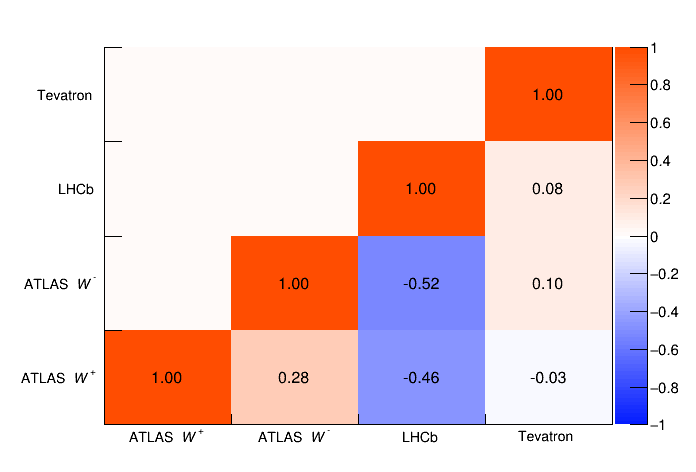
\includegraphics[width=0.9\columnwidth]{14000_CT18NNLO_ATLAS_LHCb_CDF9fb_D05fb_LEP_combination.root_rebin.png}
   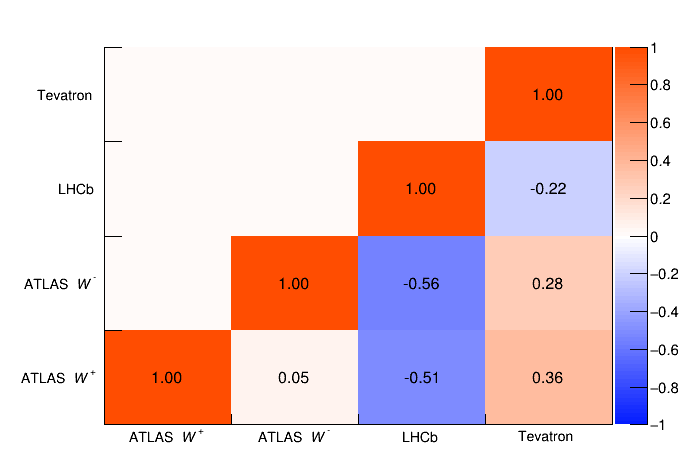
\includegraphics[width=0.9\columnwidth]{27400_MSHT20nnlo_as118_ATLAS_LHCb_CDF9fb_D05fb_LEP_combination.root_rebin.png}
   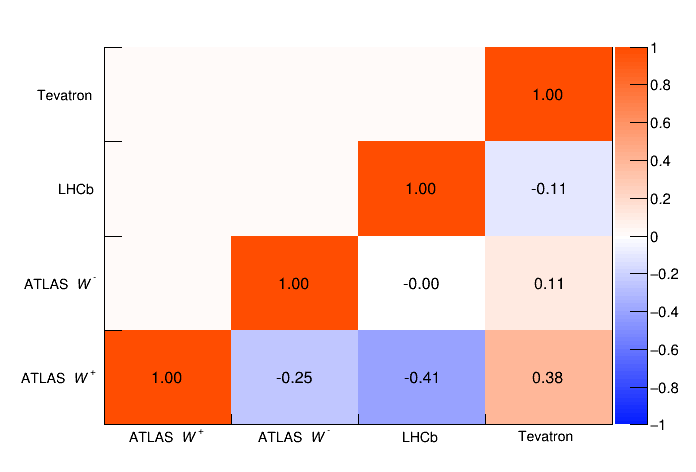
\includegraphics[width=0.9\columnwidth]{331500_NNPDF40_nnlo_as_01180_hessian_ATLAS_LHCb_CDF9fb_D05fb_LEP_combination.root_rebin.png}
   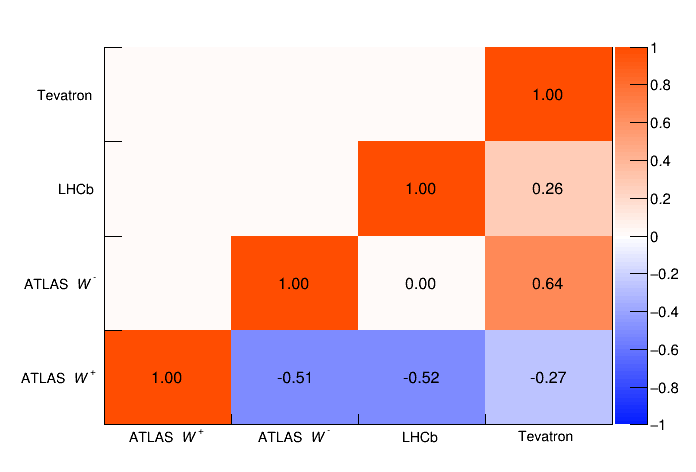
\includegraphics[width=0.9\columnwidth]{42560_ABMP16_5_nnlo_ATLAS_LHCb_CDF9fb_D05fb_LEP_combination.root_rebin.png}
   \caption{PDF uncertainty correlation matrices for the CT18, MSHT20, NNPDF4.0, and ABMP16 PDF sets, in order from top to bottom. 
}
\label{fig:pdfcorr}
\end{figure}
